\documentclass[oneside,a4]{article}                     % document properties
\usepackage[spanish, es-lcroman]{babel}                 % spanish package
\usepackage[utf8]{inputenc}                             % codificacion de caracteres utf-8
\usepackage{graphicx}                                   % Required for inserting images
\usepackage{float}                                      % float child elements
\usepackage[bottom=2.68cm,top=1.8cm,right=1.58cm,left=1.58cm]{geometry} % modify margins 
\usepackage{setspace}                                   % configure space between lines
%\usepackage{paracol}                                    % create multiple developed columns 
\usepackage{enumitem}                                   % total control of lists and its bullets
\usepackage{amsmath}                                    % math independencies
\usepackage[hidelinks]{hyperref}                        % internal links and more
\usepackage{multicol}                                   % multiple columsn
\usepackage{lipsum}                                     % lipsum random text
\usepackage{colortbl}                                   % define customize colors & table colore
\usepackage{array}                                      % customize tables  
\usepackage{rotating}                                   % allow rotate contents
\usepackage{titlesec}                                   % config auto titles
\usepackage{fancyhdr}                                   % encabezados y pies de pagina
%\usepackage{parskip}                                    % crea ambientes
\usepackage{caption}                                    % config captions
\usepackage{multirow}                                   % fusionar filas


%%%%%%%%%%%%%%%%%%%%%%%%%%%%%%%%%%%  variables  %%%%%%%%%%%%%%%%%%%%%%%%%%%%%%%
\newcommand{\itemUni}{Universidad Nacional de San Agustín}
\newcommand{\itemTheme}{Análisis Comparativo del uso de Realidad Aumentada para rehabilitación en motor fino: 4 experiencias}
\newcommand{\itemStudent}{Nombres y Apellidos Autor}
\newcommand{\itemEmail}{correo@unsa.edu.pe}
\newcommand{\itemPiePagina}{\textbf{18 LACCEI International Multi-Conference for Engineering, and Technology}: ``Engineering, Integration, and Sustainable Development'' “Hemispheric Cooperation for Competitiveness and Prosperity on a-Based Economy”, 29 July 2020, Guarena, Argentina.}


%%%%%%%%%%%%%%%%%%%%%%%%%%%%%%%%%%%  secciones y subsecciones  %%%%%%%%%%%%%%%%%%%%%%%%%%%%%%%
\titleformat{\section}[block]
  {\normalfont\small\centering}{\Roman{section}.}{1em}{\textsc}

\titleformat{\subsection}[block]
  {\normalfont\itshape}{\Alph{subsection}.}{1em}{}

\titlespacing*{\section}
  {0pt}{*1.3}{1.8mm}

\titlespacing*{\subsection}
  {0pt}{2mm}{1mm}
%%%%%%%%%%%%%%%%%%%%%%%%%%%%%%%%%%%  pies de pagina  %%%%%%%%%%%%%%%%%%%%%%%%%%%%%%%
\pagestyle{fancy}
\fancyhf{}
\renewcommand{\headrulewidth}{0pt} % Quita la línea en la cabecera
\lfoot{\footnotesize \itemPiePagina}
\rfoot{\thepage}  
%%%%%%%%%%%%%%%%%%%%%%%%%%%%%%%%%%%  titulo  %%%%%%%%%%%%%%%%%%%%%%%%%%%%%%%
\makeatletter %cambia @ para usarlo en comandos
\renewcommand{\@maketitle}{
    \begin{center}
        \begin{spacing}{2.4}
            \vspace{-0.1mm}
            \textmd{\fontsize{24}{10}\selectfont \itemTheme}\\[0.3ex]
            {\fontsize{11.3}{1}\selectfont \itemStudent$^1$,}\\[-4ex]
            {\fontsize{11.2}{1}\selectfont \textit{$^1$\itemUni, Perú, \underline{\itemEmail}}}
        \end{spacing}
    \end{center}
    \vspace{-1.06cm}
}
\makeatother %cambia @ para usarlo como caracter

\captionsetup{
  font=footnotesize,
  justification=centering,
}

\newenvironment{resumen}
{\itshape\fontsize{8}{3}\selectfont\AtBeginEnvironment{resumen}{\offinterlineskip}
\AfterEndEnvironment{resumen}{\par}}
{}
\newenvironment{tinytable}
  {\begin{center}\scriptsize}
  {\end{center}}


\newcolumntype{C}[1]{>{\centering\arraybackslash}m{#1}}
\renewcommand{\arraystretch}{1.5}
\begin{document}
    \maketitle
    \thispagestyle{fancy} % Aplicar el estilo de página en la primera página
    
    \setlength{\columnsep}{0.8cm}\begin{multicols*}{2}
        \begin{resumen}
        \textbf{Abstract} – ¿Qué se ha hecho? (Objetivo. ¿Porqué se hizo? (Problema).  Como se hizo? (Metodología). Responde a la pregunta: Porqué los resultados son útiles, importantes y a permiten ayudar a avanzar en su disciplina( Resultados)
        
        \end{resumen}
        \vspace{0.7cm}
        {\fontsize{8}{10}\selectfont\itshape 
        \textbf{Keywords-- List at most 5 key index terms here.}
        
        }\vspace{0.45cm}
        
    \section{Introducción}

\%El primer párrafo presenta información general sobre el tema en estudio o problema que se trata de resolver. Debe resaltar la importancia del tema tratado. y su impacto\%

\%El Segundo párrafo resalta las investigaciones previas\%

\%El tercer párrafo resalta el trabajo desarrollado , que se ha hecho (mencionar los casos) y como se hizo\%

\%El cuarto párrafo presenta la estructura del artículo. Siempre inicia con las palabras: ``El resto del artículo está organizado de la siguiente manera...'' \%


\section{Tema 1 – Realidad Aumentada}

\subsection{Definición y conceptos fundamentales}
Use automatic hyphenation and check spelling and grammar. Use high resolution (300dpi or above) figures, plots, drawings and photos for best printing result.

\subsection{Enfoques terapéuticos}
Use automatic hyphenation and check spelling and grammar. Use high resolution (300dpi or above) figures, plots, drawings and photos for best printing result.

\subsection{Desafíos y limitaciones}
Use automatic hyphenation and check spelling and grammar. Use high resolution (300dpi or above) figures, plots, drawings and photos for best printing result.


\section{Tema 2 – Marco Teórico}
\subsection{Subtema 1}
Use automatic hyphenation and check spelling and grammar. Use high resolution (300dpi or above) figures, plots, drawings and photos for best printing result.

\subsection{Subtema 2}
Use automatic hyphenation and check spelling and grammar. Use high resolution (300dpi or above) figures, plots, drawings and photos for best printing result.

\subsection{Subtema 3}
Use automatic hyphenation and check spelling and grammar. Use high resolution (300dpi or above) figures, plots, drawings and photos for best printing result.

\section{Metodología}

\subsection{Caso 1}

En el trabajo de Coronado et al. [10], se presenta el uso de la tecnología de Realidad Virtual (RV) en un sistema de control de balance para pacientes con Parkinson. El sistema utiliza el dispositivo Oculus, el cual proporciona una experiencia inmersiva a través de una simulación de bicicleta en un entorno virtual con un camino, árboles y obstáculos que deben ser evitados mediante el movimiento del cuerpo hacia la izquierda o derecha, respectivamente (Figura 4). Para la captura de los movimientos corporales, se integró el controlador Leap Motion Controller. El estudio se llevó a cabo en el Hospital Honorio Delgado, específicamente en el área de neurología.\\

Diez pacientes con enfermedad de Parkinson en estados iniciales participaron en el estudio, compuesto por cinco hombres y cinco mujeres, con edades comprendidas entre 55 y 78 años. El protocolo del estudio consistió en diez sesiones de intervención, realizadas tres veces por semana, con una duración de 30 minutos cada sesión.\\

Antes y después de las sesiones, se evaluó el desempeño de los pacientes utilizando pruebas clínicas, específicamente el Test de la Batería de Evaluación del Movimiento (BOT-2) [11] y el Test de Bloques y Cajas (Block and Box Test) [12]. Además, se recopiló la opinión de los pacientes sobre la usabilidad del sistema mediante cuestionarios de evaluación de satisfacción del usuario (User Satisfaction Evaluation Questionnaire, USEQ) [13], cuestionarios de experiencia del usuario (User Experience Questionnaire, UEQ) [14] y el Modelo de Aceptación Tecnológica (Technological Acceptance Model, TAM) [15].\\

Los resultados obtenidos mostraron una mejora significativa en la subprueba del balance del Test BOT-2 en ocho de los participantes, evidenciando los beneficios del sistema de control de balance basado en Realidad Virtual. Dos participantes no mostraron mejoría en esta área específica. En cuanto a las opiniones de los pacientes, cinco de ellos manifestaron que disfrutaron de la experiencia proporcionada por el sistema RV, mientras que los otros cinco experimentaron mareos después de utilizar el dispositivo. Los resultados del cuestionario UEQ revelaron una valoración positiva por encima de los 4 puntos, lo cual indica una alta aceptación del sistema por parte de los usuarios.


\subsection{Caso 2}
Se describe el contexto (institución y lugar), tiempo que duró la experiencia, cantidad de participantes, resultados obtenidos, software/hardware/metodología utilizados (según corresponda)

\subsection{Caso 3}
Se describe el contexto (institución y lugar), tiempo que duró la experiencia, cantidad de participantes, resultados obtenidos, software/hardware/metodología utilizados (según corresponda)

\subsection{Caso 4}
Se describe el contexto (institución y lugar), tiempo que duró la experiencia, cantidad de participantes, resultados obtenidos, software/hardware/metodología utilizados (según corresponda)
 
\section{Resultados y Discusión}
En el análisis comparativo de los cuatro casos de uso de realidad aumentada para rehabilitación en motor fino, se identificaron semejanzas y diferencias relevantes.

\subsection{Semejanzas}
Use automatic hyphenation and check spelling and grammar. Use high resolution (300dpi or above) figures, plots, drawings and photos for best printing result.

\subsection{Diferencias}
Use automatic hyphenation and check spelling and grammar. Use high resolution (300dpi or above) figures, plots, drawings and photos for best printing result.

\subsection{Discusión}
Use automatic hyphenation and check spelling and grammar. Use high resolution (300dpi or above) figures, plots, drawings and photos for best printing result.

\subsection{Propuesta}
Use automatic hyphenation and check spelling and grammar. Use high resolution (300dpi or above) figures, plots, drawings and photos for best printing result.

\section{Conclusiones}
    \vspace{1cm}
    \begin{thebibliography}{X}
    \bibitem{Manuscript} Manuscript Templates for Conference Proceedings, IEEE. \url{http://www.ieee.org/conferences_events/conferences/publishing/templates.html}
    \bibitem{King} M. King, B. Zhu, and S. Tang, ``Optimal path planning,'' Mobile Robots, vol. 8, no. 2, pp. 520-531, March 2001.
    \bibitem{Simpson} H. Simpson, Dumb Robots, 3rd ed., Springfield: UOS Press, 2004, pp.6-9.
    \bibitem{King2} M. King and B. Zhu, ``Gaming strategies,'' in Path Planning to the West, vol. II, S. Tang and M. King, Eds. Xian: Jiaoda Press, 1998, pp. 158-176.
    \bibitem{Simpson2} B. Simpson, et al, ``Title of paper goes here if known,'' unpublished.
    \bibitem{Lu} J.-G. Lu, ``Title of paper with only the first word capitalized,'' J. Name Stand. Abbrev., in press.
    \bibitem{Yorozu} Y. Yorozu, M. Hirano, K. Oka, and Y. Tagawa, ``Electron spectroscopy studies on magneto-optical media and plastic substrate interface,'' IEEE Translated J. Magn. Japan, vol. 2, pp. 740-741, August 1987 [Digest 9th Annual Conf. Magnetics Japan, p. 301, 1982]. 
    \bibitem{Young} M. Young, The Technical Writer’s Handbook, Mill Valley, CA: University Science, 1989.
\end{thebibliography}    

    \section{Anexos}

    \begin{tinytable}
        \begin{tabular}{|C{1.2cm}|p{2cm}|p{1.2cm}|p{1.5cm}|}
        \hline
            \multirow{2}{1cm}{Type Size (pts.)} & \multicolumn{3}{c|}{Apperance} \\ [10pt]\cline{2-4}
            & Regular & Bold & Italic\\\hline
            6 & Table superscripts &  & \\\hline
            8 & Section titles, references, tables, table names, table captions, figure captions, footnotes, text subscripts, and superscripts &  & \\\hline
            9 &  & Abstract, Index Terms & \\\hline
            10 & Authors affiliations, main text, equations, first letter in section titles &  & Subheading  \\\hline
            11 & Authors names &  & \\\hline
            12 & Paper title &  & \\\hline
        \end{tabular}
        \captionof{table}{This is a simple table}
    \end{tinytable}
    
    
    \begin{figure}[H]
        \centering
        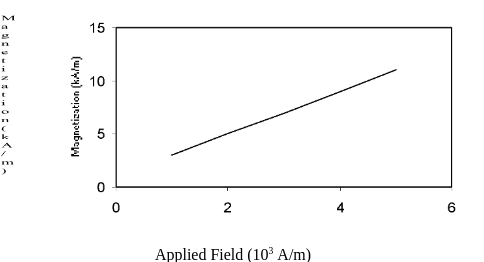
\includegraphics[width=0.9\linewidth]{images/imagen.png}
        \caption{Magnetization as a function of applied field. Note caption is centered below figures, but above tables.}
    \end{figure}
    
    \end{multicols*}
\end{document}
